\chapter{First Hop Redundancy
Protocols}\label{first-hop-redundancy-protocols}

\section{The Purpose of FHRPs}\label{the-purpose-of-fhrps}

\begin{figure}
\centering
\pandocbounded{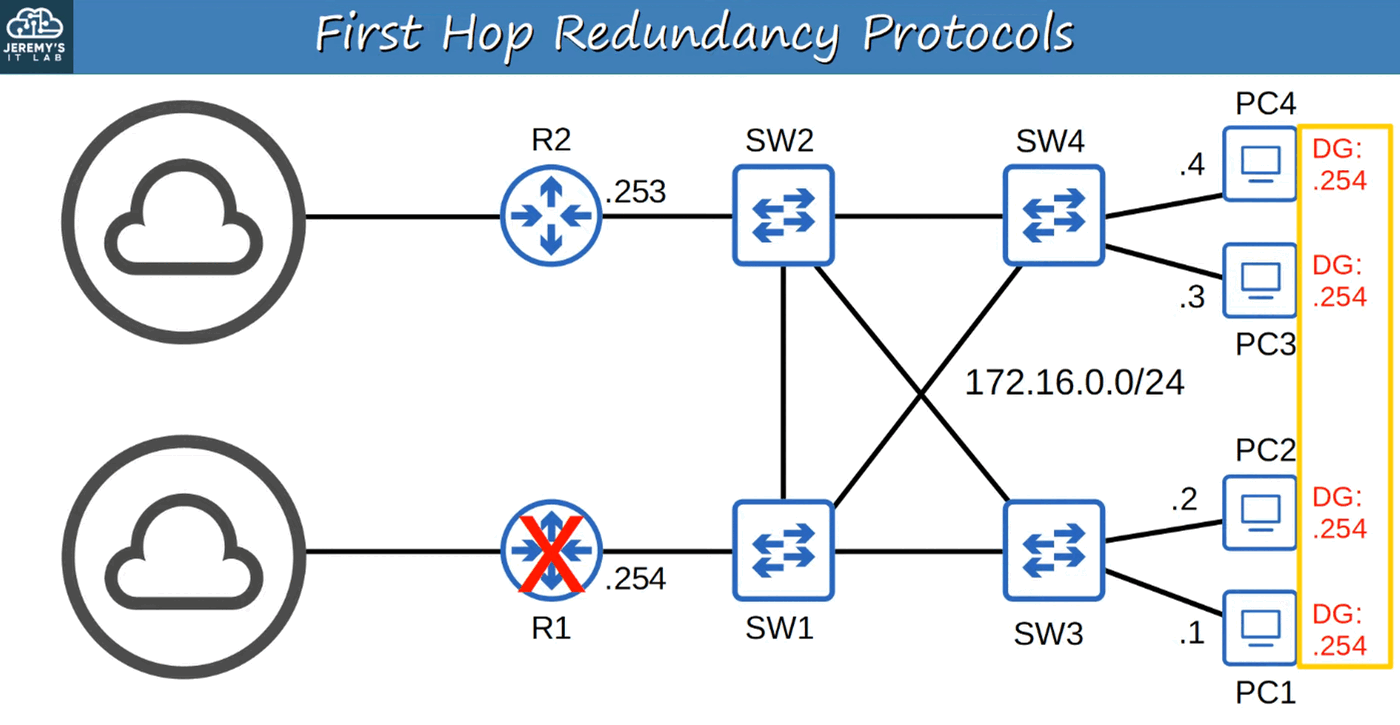
\includegraphics[keepaspectratio,alt={image}]{images/30-first-hop-redundancy-protocols/img-001.png}}
\end{figure}

What happens when the configured DEFAULT GATEWAY for network HOSTS goes
down ?

What happens to the routed traffic?

How can we route our traffic to the functional GATEWAY at R2 (.253) ?

This is what the FIRST HOP REDUNDANCY PROTOCOL is designed to fix

\section{First Hop Redundancy Protocol
(FHRP)}\label{first-hop-redundancy-protocol-fhrp}

\begin{itemize}
\tightlist
\item
  Computer networking protocol
\item
  Designed to PROTECT the DEFAULT GATEWAY used on a SUBNET by allowing
  TWO or MORE ROUTERS to provide BACKUP for that ADDRESS
\item
  In the event of a FAILURE of the ACTIVE ROUTER, the BACKUP ROUTER will
  take over the ADDRESS (usually within seconds)
\end{itemize}

HOW DOES FHRP WORK?

\begin{itemize}
\tightlist
\item
  TWO (or more) ROUTERS share a VIP (A Virtual IP ADDRESS)
\item
  THIS VIP is used by HOSTS as the DEFAULY GATEWAY IP
\item
  The ROUTERS communicate with each other by sending ``Hello'' messages
\item
  One ROUTER becomes the ACTIVE ROUTER, the other(s) STANDBY
\item
  When a HOST sends traffic to an ADDRESS outside of the NETWORK, it
  sends an ARP REQUEST (Broadcast Flood) to the VIP to find out it's MAC
  ADDRESS

  \begin{itemize}
  \tightlist
  \item
    Spanning Tree prevents BROADCAST STORM due to Broadcast Flood
  \end{itemize}
\item
  The ACTIVE ROUTER sends the ARP REPLY back (it's VIRTUAL MAC ADDRESS)
  to the HOST
\item
  The HOST now sends traffic OUTSIDE of the NETWORK with:

  \begin{itemize}
  \tightlist
  \item
    Source IP (HOST IP)
  \item
    Destination IP (External IP ADDRESS)
  \item
    Source MAC (HOST MAC ADDRESS)
  \item
    Destination MAC (GATEWAY VIP MAC ADDRESS)
  \end{itemize}
\end{itemize}

\begin{figure}
\centering
\pandocbounded{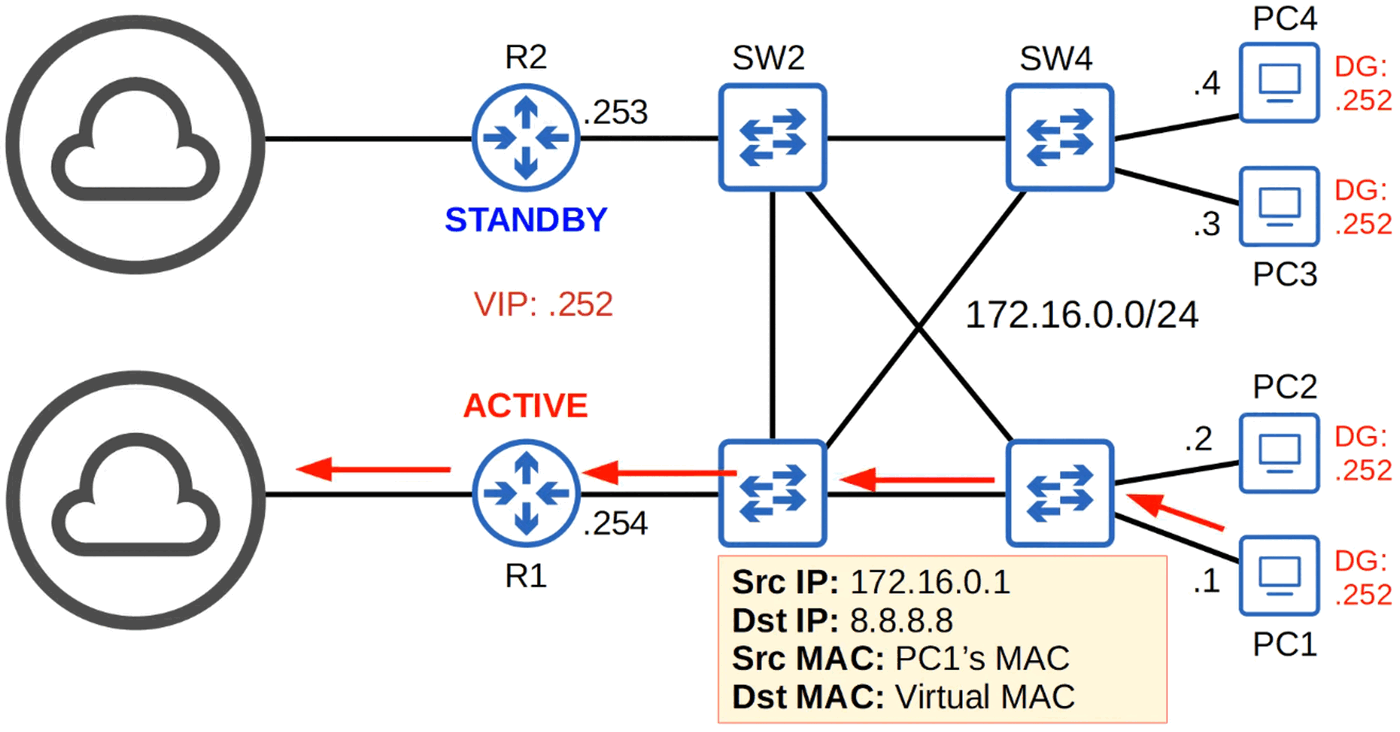
\includegraphics[keepaspectratio,alt={image}]{images/30-first-hop-redundancy-protocols/img-002.png}}
\end{figure}

IF R1 goes down, R2 will switch from STANDY to ACTIVE after not
receiving ``Hello'' messages from R1

\begin{figure}
\centering
\pandocbounded{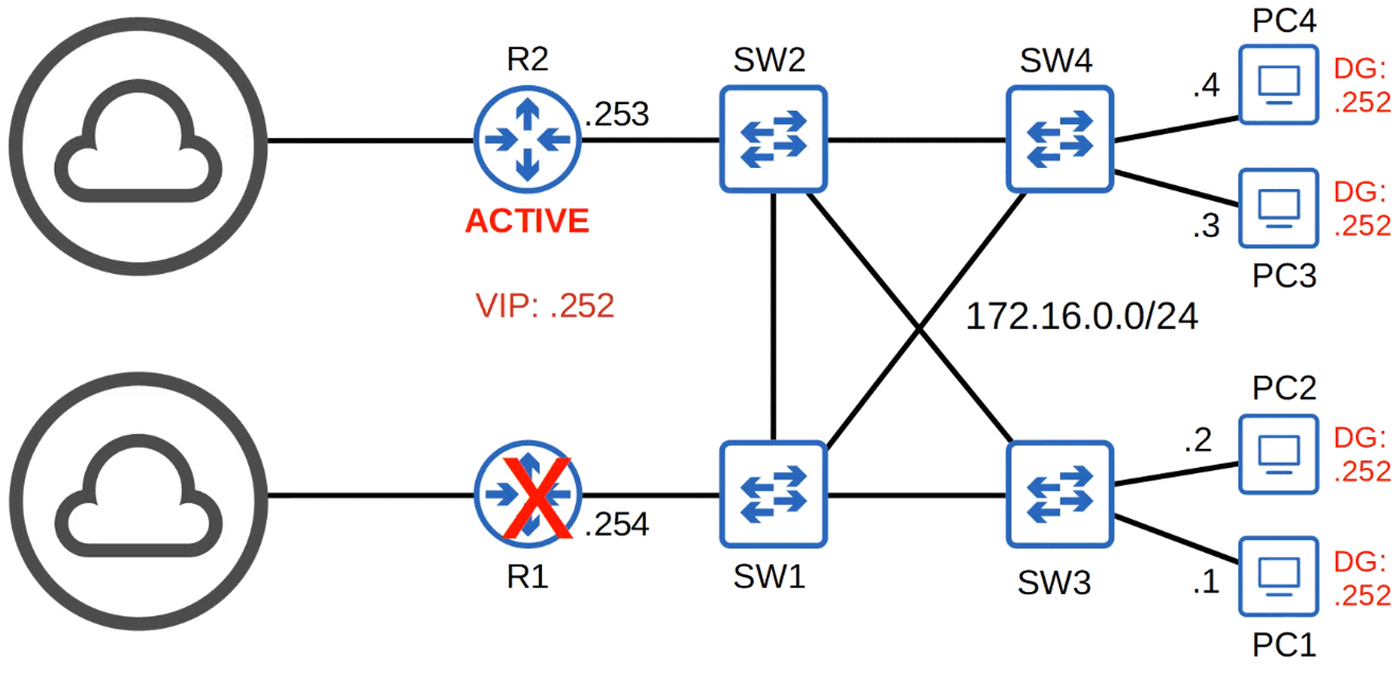
\includegraphics[keepaspectratio,alt={image}]{images/30-first-hop-redundancy-protocols/img-003.png}}
\end{figure}

The HOST ARP TABLE doesn't need to change since the MAC ADDRESS of the
VIP is already known and traffic flows externally via R2

R2 DOES need to update the SWITCHES with a GRATUITOUS ARP

\begin{itemize}
\tightlist
\item
  GRATUITOUS ARP is an ARP REPLY sent without being REQUESTED (no ARP
  REQUEST received)
\item
  GRATUITOUS ARP uses BROADCAST (FFFF.FFFF.FFFF) - Normal ARP REPLY is
  Unicast
\end{itemize}

\begin{figure}
\centering
\pandocbounded{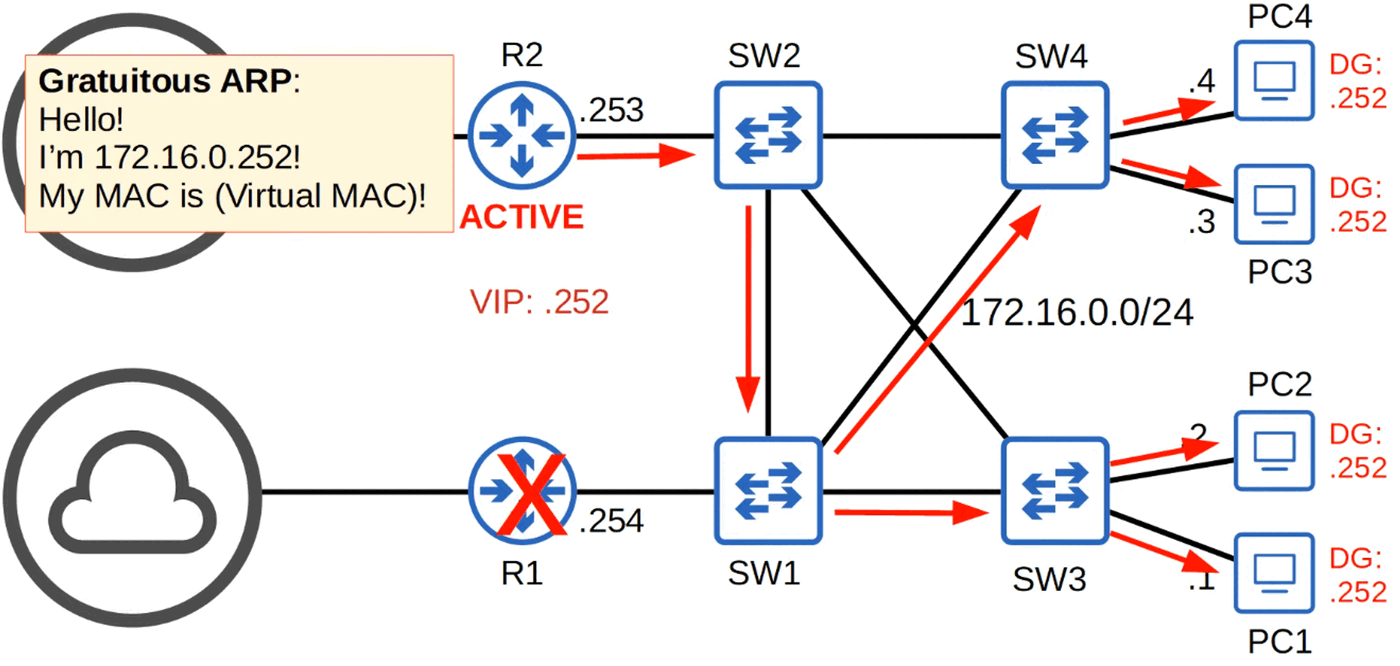
\includegraphics[keepaspectratio,alt={image}]{images/30-first-hop-redundancy-protocols/img-004.png}}
\end{figure}

\begin{figure}
\centering
\pandocbounded{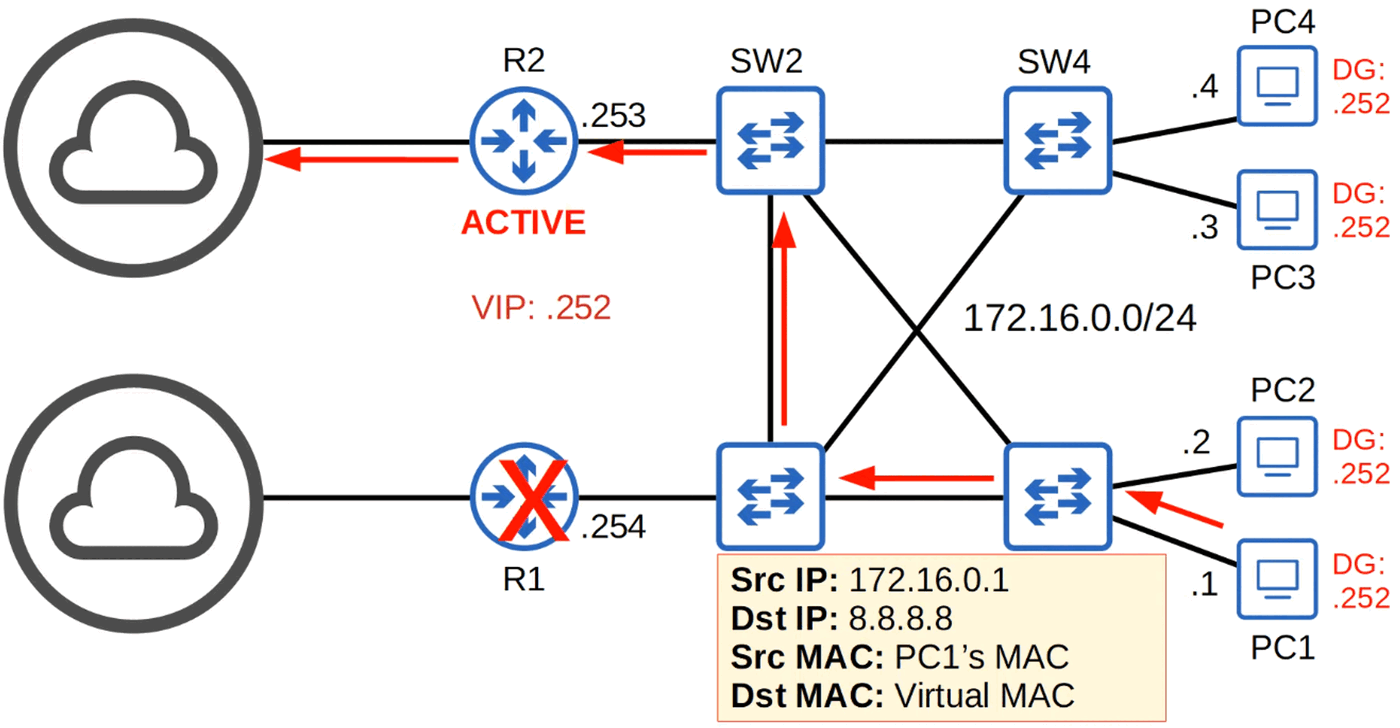
\includegraphics[keepaspectratio,alt={image}]{images/30-first-hop-redundancy-protocols/img-005.png}}
\end{figure}

What happens is R1 comes back ONLINE again?

It becomes a STANDBY ROUTER

R2 remains the ACTIVE ROUTER

\begin{tipbox}

FPRPs are ``non-preemptive''. The current ACTIVE ROUTER will not
automatically give up its role, even if the former ACTIVE ROUTER
returns.

*** You CAN change this setting to make R1 `preempt' R2 and take back
it's ACTIVE role, automatically ***

\end{tipbox}

\section{HSRP (Hot Standby Router
Protocol)}\label{hsrp-hot-standby-router-protocol}

\begin{itemize}
\tightlist
\item
  \textbf{Cisco proprietary}
\item
  An ACTIVE and STANDBY ROUTER are elected
\item
  There are TWO VERSIONS :

  \begin{itemize}
  \tightlist
  \item
    version 1
  \item
    version 2 : \emph{adds IPv6 support} and increases \# of
    \emph{groups} that can be configured
  \end{itemize}
\item
  Multicast IPv4 ADDRESSES :

  \begin{itemize}
  \tightlist
  \item
    \textbf{v1} : 224.0.0.2
  \item
    \textbf{v2} : 224.0.0.102
  \end{itemize}
\item
  VIRTUAL MAC ADDRESSES :

  \begin{itemize}
  \tightlist
  \item
    \textbf{v1} : 0000.0c07.acXX (XX = HSRP GROUP NUMBER)
  \item
    \textbf{v2} : 0000.0c9f.fXXX (XXX = HSRP GROUP NUMBER)
  \end{itemize}
\item
  In a situation with MULTIPLE SUBNETS / VLANS, you can configure a
  DIFFERENT ACTIVE ROUTER in EACH SUBNET / VLAN to LOAD BALANCE
\end{itemize}

\begin{figure}
\centering
\pandocbounded{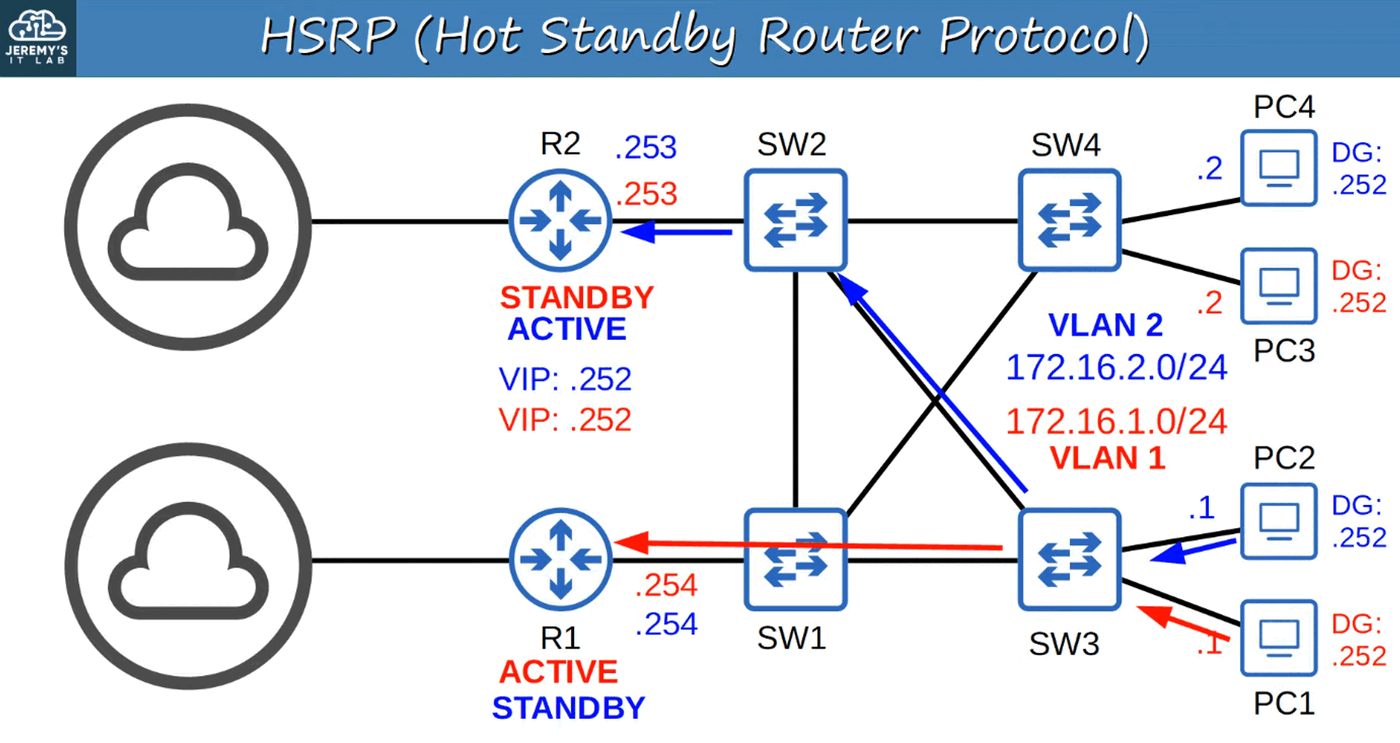
\includegraphics[keepaspectratio,alt={image}]{images/30-first-hop-redundancy-protocols/img-006.png}}
\end{figure}

\section{VRRP (Virtual Router Redundancy
Protocol)}\label{vrrp-virtual-router-redundancy-protocol}

\begin{itemize}
\item
  Open Standard
\item
  A MASTER and BACKUP ROUTER are elected
\item
  Multicast IPv4 ADDRESSES :

  \begin{itemize}
  \tightlist
  \item
    224.0.0.18
  \end{itemize}
\item
  VIRTUAL MAC ADDRESSES :

  \begin{itemize}
  \tightlist
  \item
    0000.5e00.01XX (XX = VRRP GROUP NUMBER)

    \begin{itemize}
    \tightlist
    \item
      for GROUP NUMBERS \textgreater{} 99, you need to convert the
      number to HEX
    \item
      Example: 200 = ``c8'' in Hex so the MAC would be 0000.5e00.01c8
    \end{itemize}
  \end{itemize}
\item
  In a situation with MULTIPLE SUBNETS / VLANS, you can configure a
  DIFFERENT MASTER ROUTER in EACH SUBNET / VLAN to LOAD BALANCE
\end{itemize}

\begin{figure}
\centering
\pandocbounded{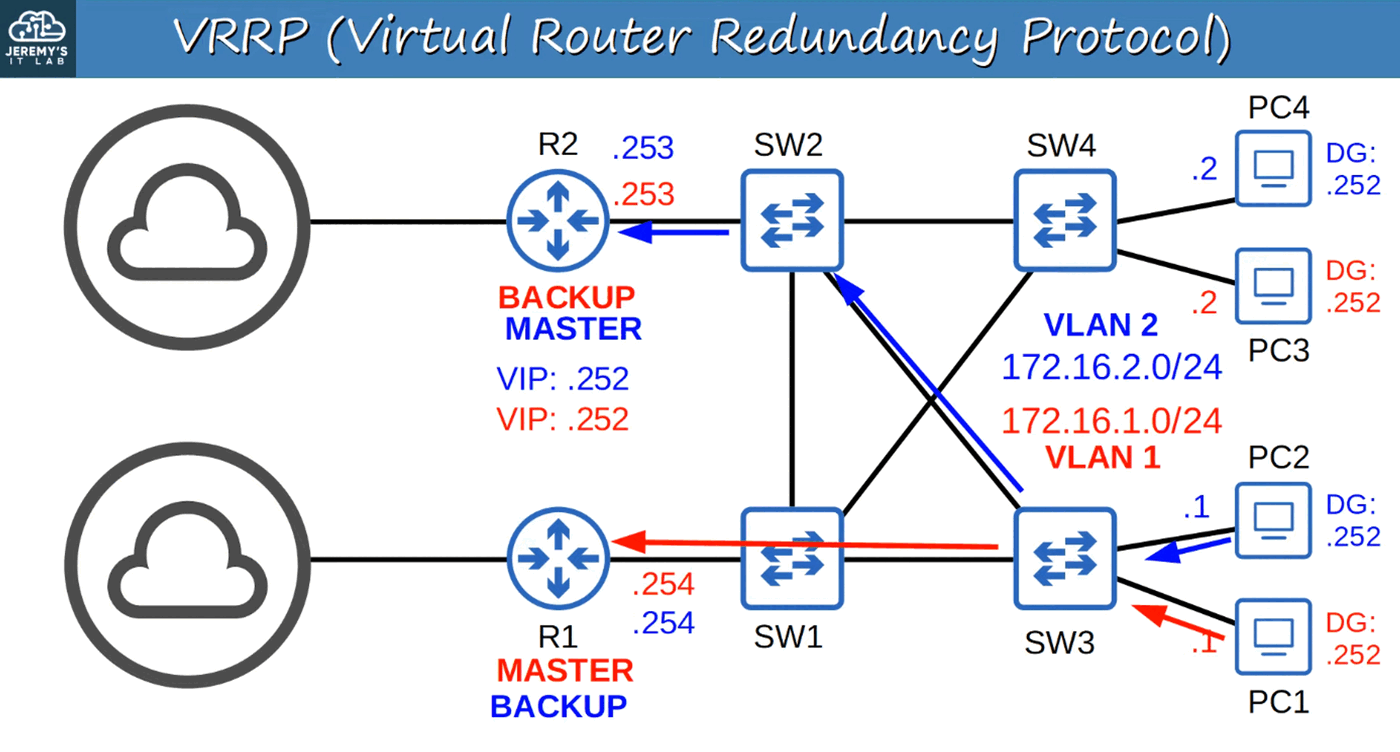
\includegraphics[keepaspectratio,alt={image}]{images/30-first-hop-redundancy-protocols/img-007.png}}
\end{figure}

\section{GLBP (Gateway Load Balancing
Protocol)}\label{glbp-gateway-load-balancing-protocol}

\begin{itemize}
\item
  Cisco Proprietary
\item
  LOAD BALANCES among MULTIPLE ROUTERS within a SINGLE SUBNET
\item
  An AVG (Active Virtual Gateway) is elected
\item
  Up to FOUR AVFs (Active Virtual Forwarders) are assigned BY the AVG
  (the AVG can be an AVF, too)
\item
  Each AVF acts as the DEFAULT GATEWAY for a portion of the HOSTS in the
  SUBNET
\item
  Multicast IPv4 ADDRESSES :

  \begin{itemize}
  \tightlist
  \item
    224.0.0.102
  \end{itemize}
\item
  VIRTUAL MAC ADDRESSES :

  \begin{itemize}
  \tightlist
  \item
    0007.b400.XXYY (XX = GLBP GROUP NUMBER, YY = AVF NUMBER)
  \end{itemize}
\end{itemize}

MEMORIZE THIS CHART and the differences between the FHRPs

\begin{figure}
\centering
\pandocbounded{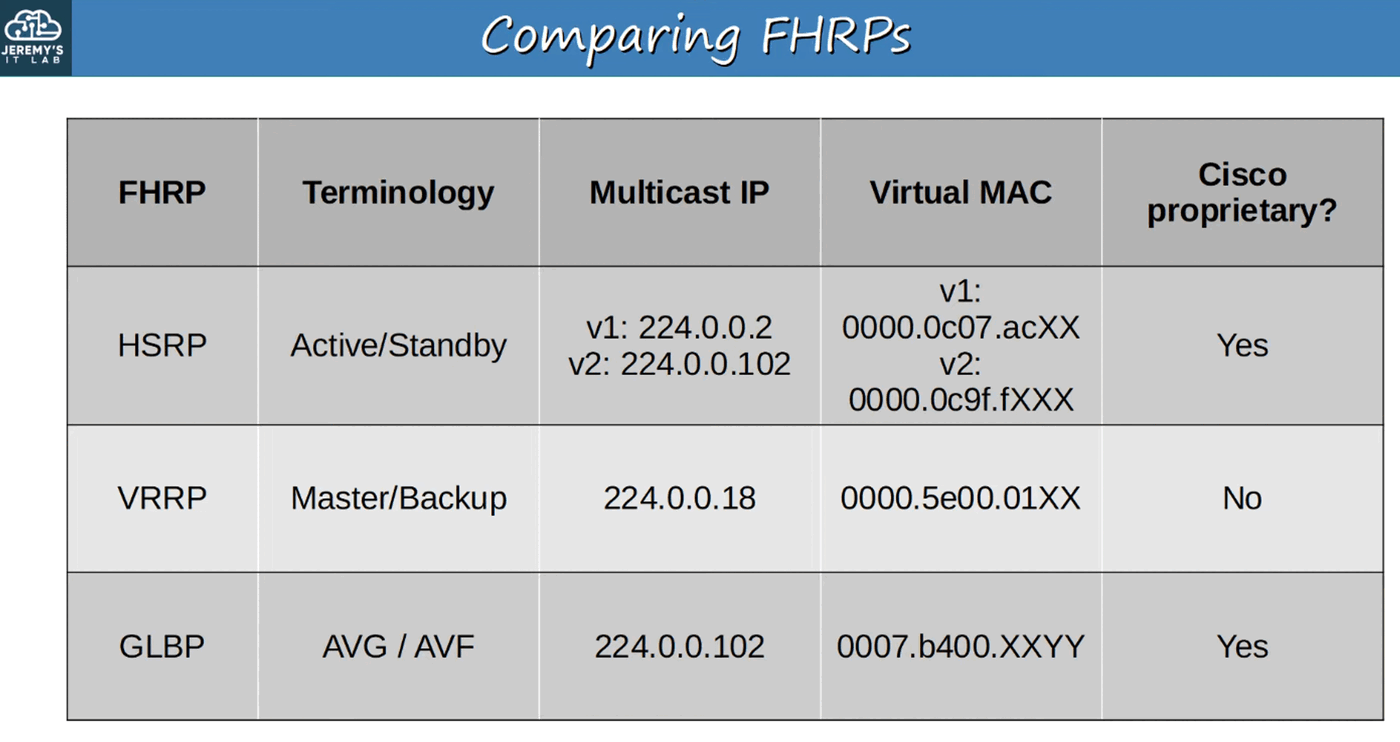
\includegraphics[keepaspectratio,alt={image}]{images/30-first-hop-redundancy-protocols/img-008.png}}
\end{figure}

\section{Basic HSRP Configuration}\label{basic-hsrp-configuration}

R1s configuration

\begin{figure}
\centering
\pandocbounded{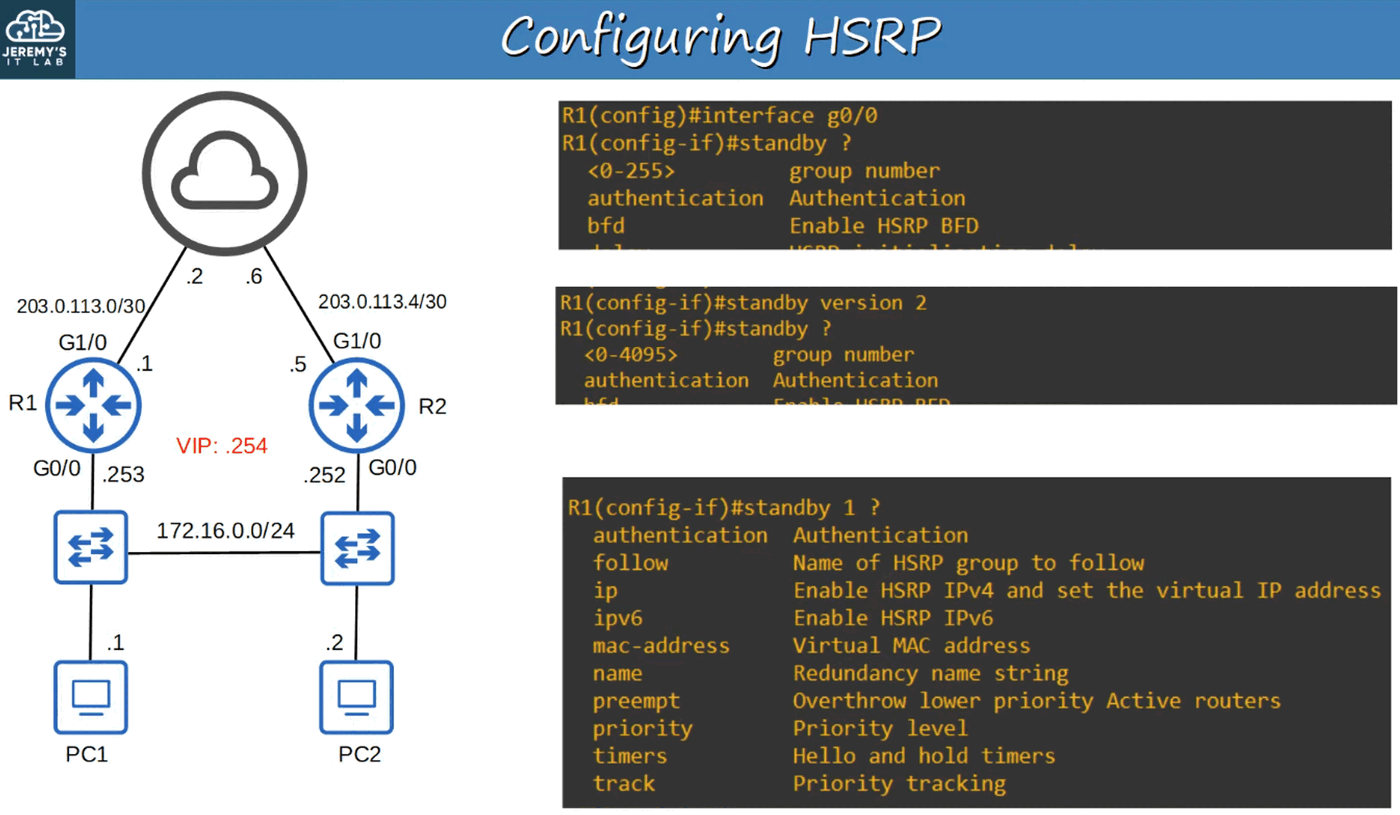
\includegraphics[keepaspectratio,alt={image}]{images/30-first-hop-redundancy-protocols/img-009.png}}
\end{figure}

NOTE : group number has to match ALL ROUTERS being configured in a given
SUBNET

\begin{figure}
\centering
\pandocbounded{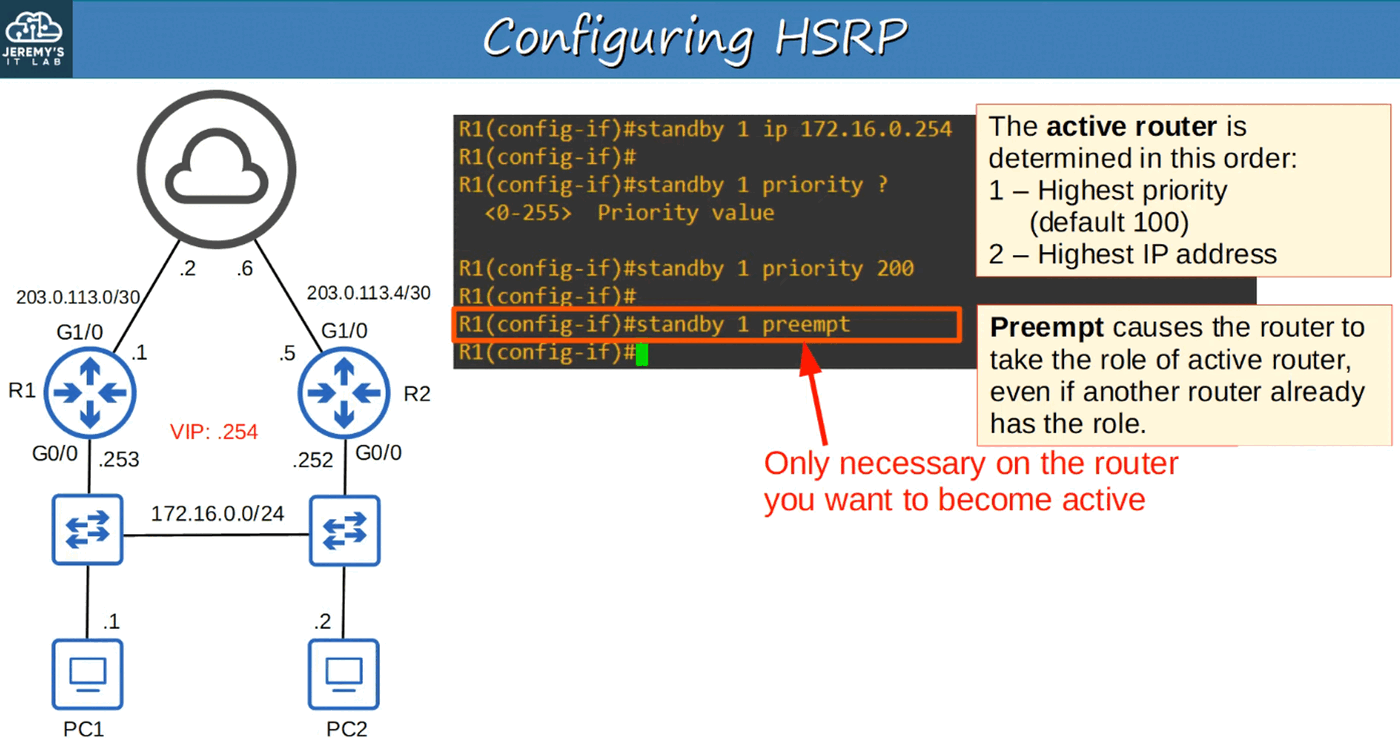
\includegraphics[keepaspectratio,alt={image}]{images/30-first-hop-redundancy-protocols/img-010.png}}
\end{figure}

R2's configuration

\begin{figure}
\centering
\pandocbounded{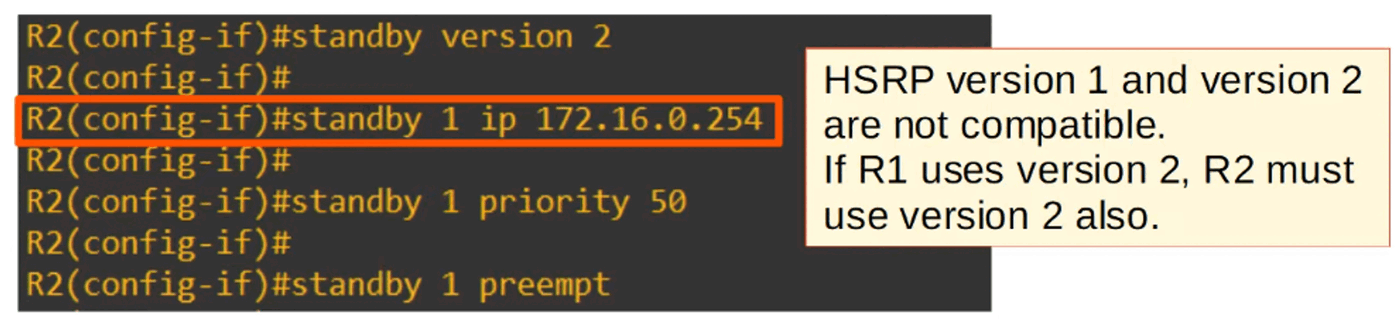
\includegraphics[keepaspectratio,alt={image}]{images/30-first-hop-redundancy-protocols/img-011.png}}
\end{figure}

NOTE : HSRP versions are not cross-compatible. All ROUTERS must use the
same HSRP Version

Output of the ``show standby'' command

\begin{figure}
\centering
\pandocbounded{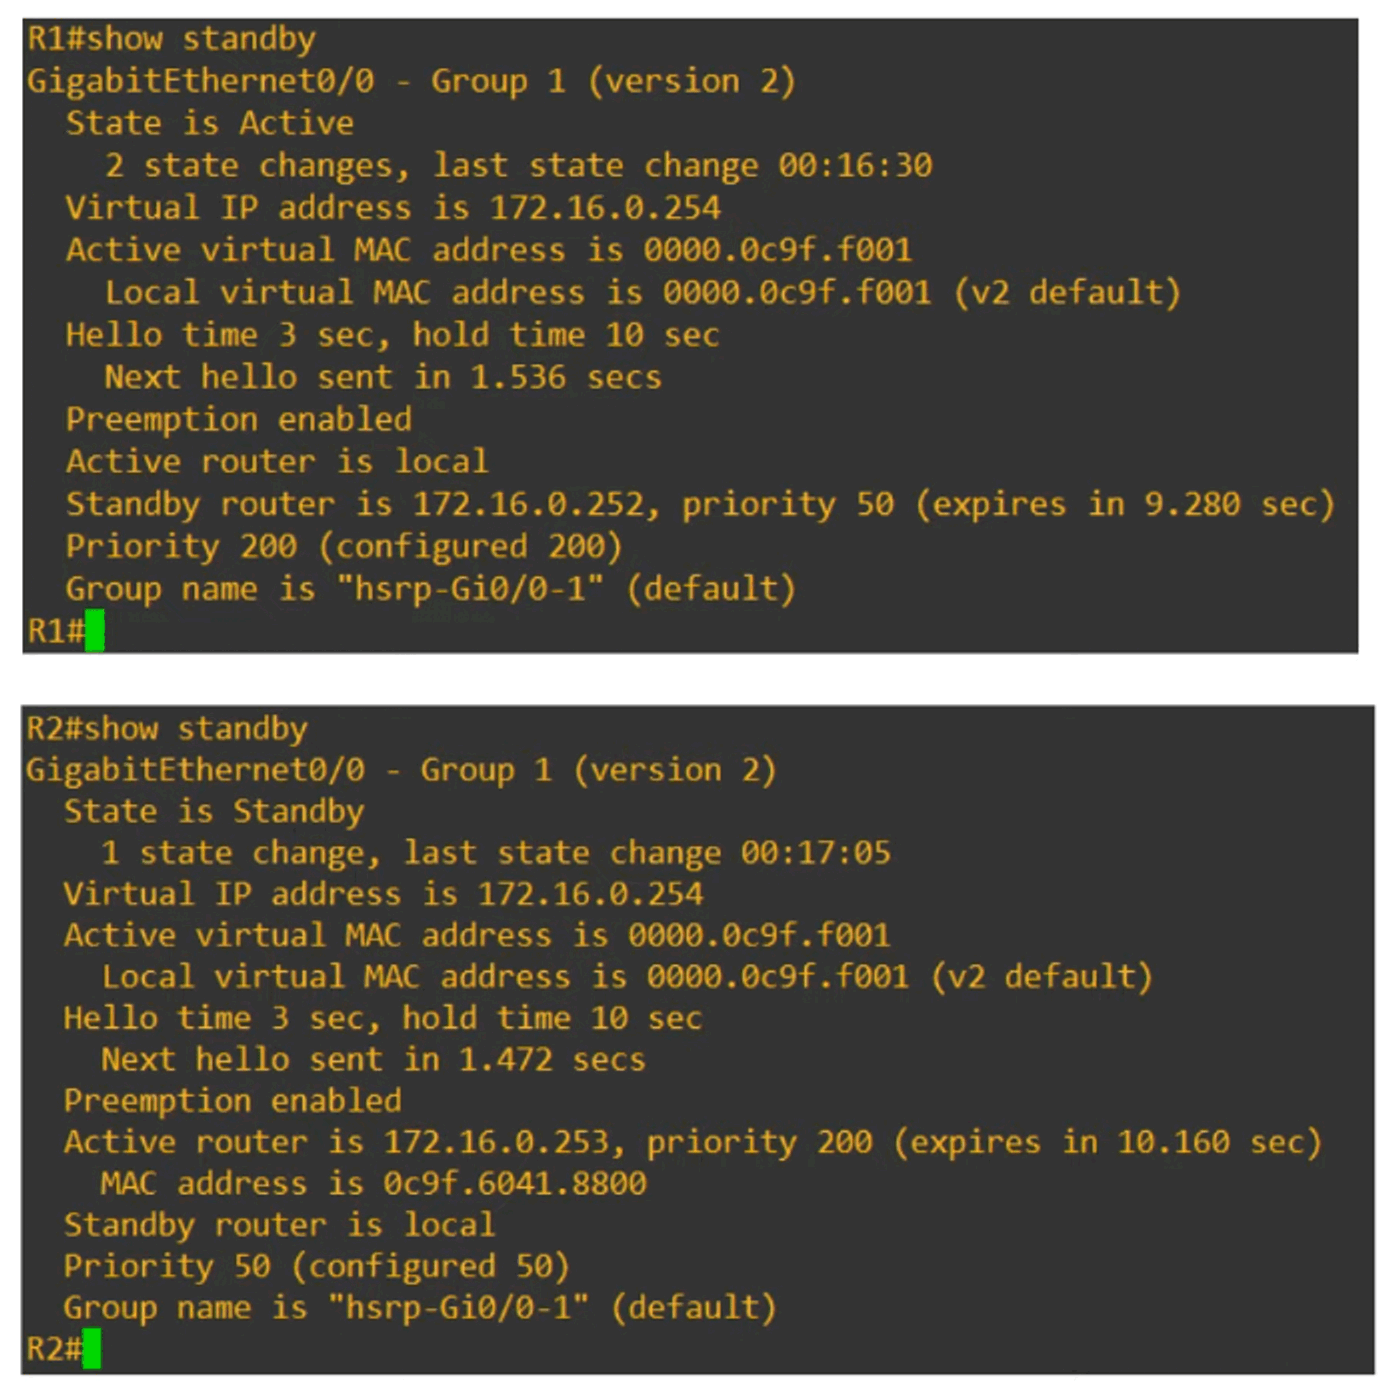
\includegraphics[keepaspectratio,alt={image}]{images/30-first-hop-redundancy-protocols/img-012.png}}
\end{figure}
